		\begin{table} % Table 1
		\centering
		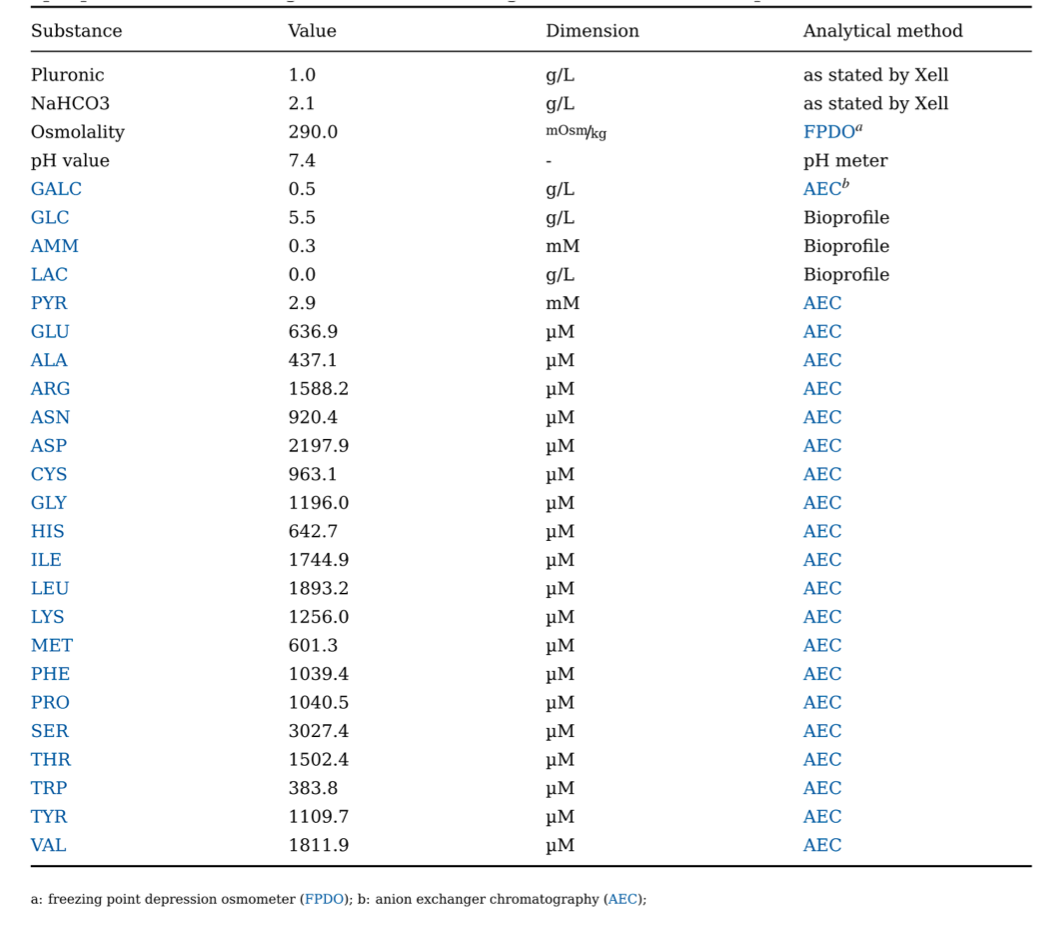
\includegraphics[scale = 0.68]{Table_3_1}
		\caption{Measured medium composition of the 42-MAX-UB standard medium. Extracted from \protect\cite{Rath2017a}}
		
	\end{table}
	
	\begin{table} % Table 2
		\centering
		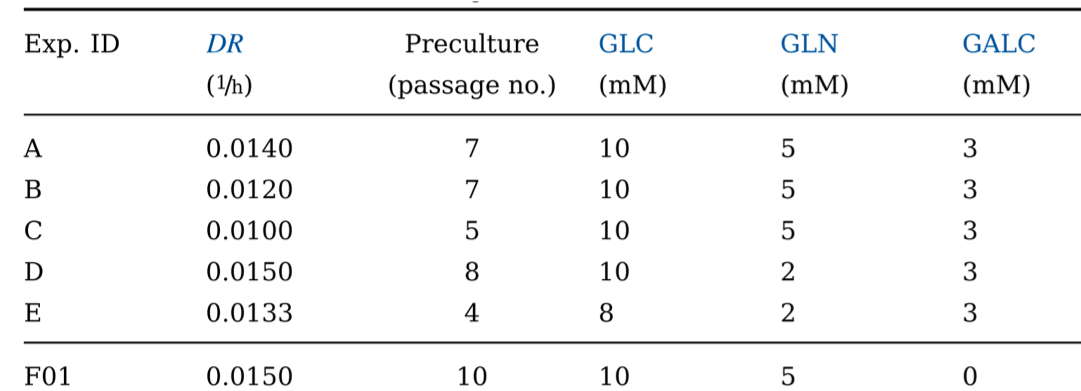
\includegraphics[scale = 0.63]{Table_4_10}
		\caption{The dilution rates, preculture ages and the 42-Max-UB-medium modified components concentrations used in \protect\cite{Rath2017a} for the 6 steady states. Table adapted from \protect\cite{Rath2017a}}
		
	\end{table}
	
	\begin{sidewaystable} % Table 3
		\centering
		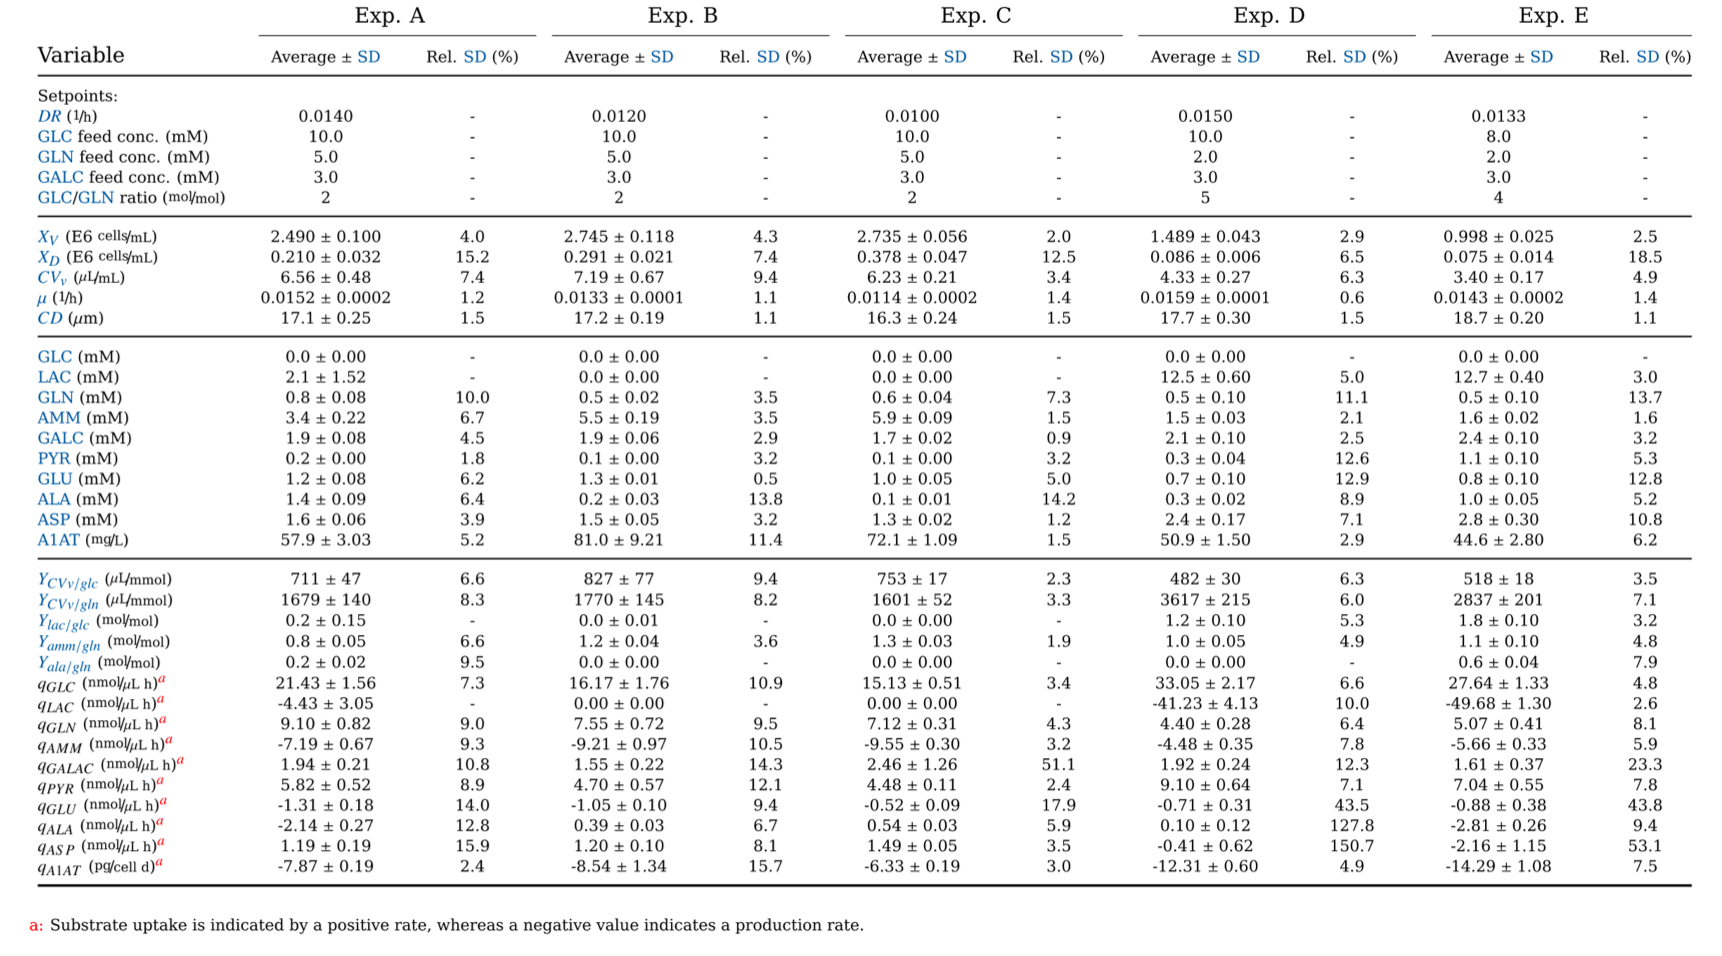
\includegraphics[scale = 0.7]{Table_4_11}
		\caption{Steady-state values reported for \protect\cite{Rath2017a} of different parameters from continuous cultivations with varying GLC and GLN feed concentrations and with 3 mM GAL. Table taken from \protect\cite{Rath2017a}}
		
	\end{sidewaystable}
	
	\begin{table} % Table 4
		\centering
		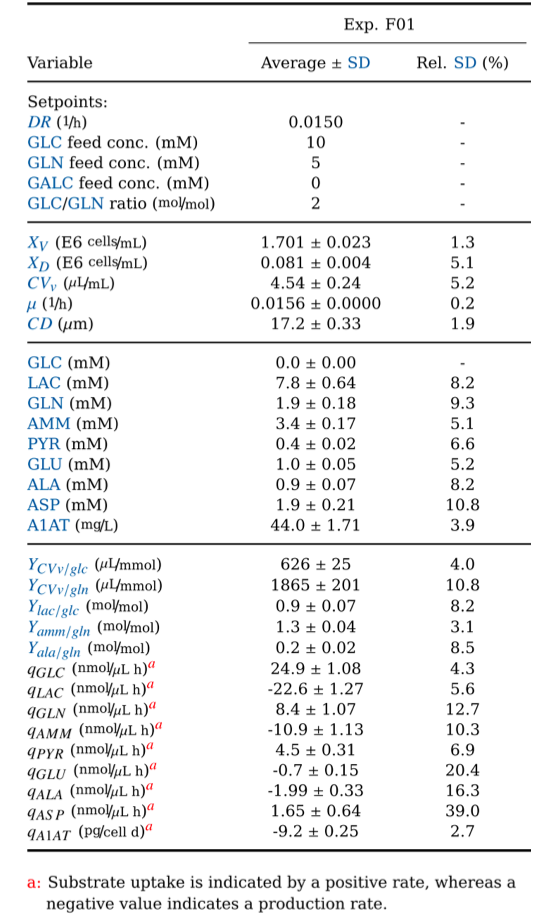
\includegraphics[scale = 0.8]{Table_4_12}
		\caption{Steady-state values reported for \protect\cite{Rath2017a} of different parameters from continuous cultivations with varying GLC and GLN feed concentrations and without GAL. Table taken from \protect\cite{Rath2017a}}
		
	\end{table}